\section{ARROW}
\label{sec:method}

\begin{figure*}[t]
  \centering
  \IfFileExists{figures/fig2_method_ownership.pdf}{%
    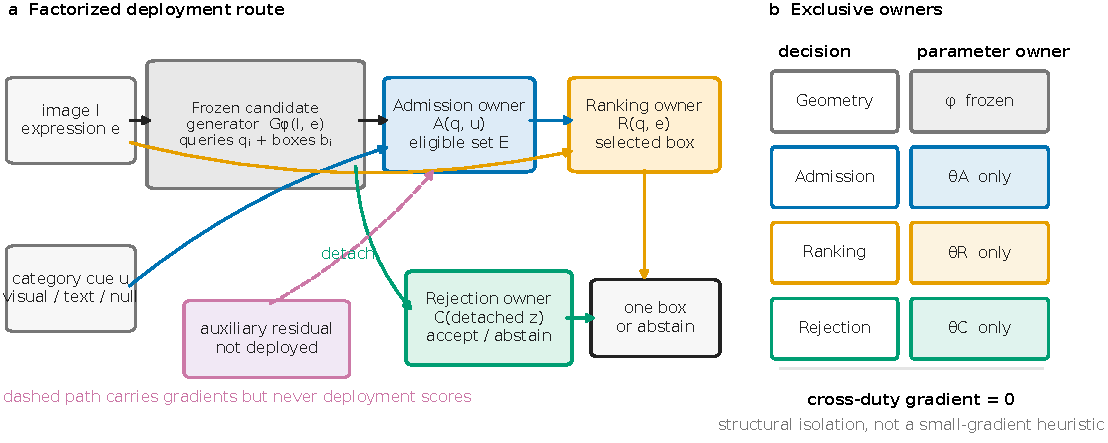
\includegraphics[width=\textwidth]{figures/fig2_method_ownership.pdf}%
  }{\fbox{\parbox[c][1.35in][c]{0.96\textwidth}{\centering
    Frozen candidates $\rightarrow$ Admission $\rightarrow$ Ranking; detached
    evidence $\rightarrow$ Abstention.}}}
  \caption{\method factorizes the deployed policy without prescribing one
  universal parameter topology.  Admission defines the comparison set,
  Ranking selects within it, and Abstention decides whether the selected box is
  emitted.  ARROW-U2 isolates Ranking and Abstention; matched controls test
  shared and isolated owner allocations.  The auxiliary Admission residual is
  serialized and computed for compatibility but ignored by every deployed
  decision score.}
  \label{fig:method}
\end{figure*}

\subsection{Frozen full-expression candidates}
\method retains the full-expression Grounding DINO candidate generator.  The
complete expression always enters the language encoder, transformer, decoder,
and box predictor; neither a canonical noun nor a generic ``object'' prompt
replaces this geometry path.  The frozen generator returns boxes $b_i$,
final-decoder queries $h_i$, and native scores $s_i^0$.  Freezing keeps
candidate geometry and base evidence identical across cue and owner controls.

\subsection{Category-conditioned Admission}
Let $u$ denote the category cue.  Admission computes
$\bar u=P_{\theta_A}(u)$ and
\begin{equation}
  a_i=\alpha\cos(W_{\theta_A}h_i,\bar u).
\end{equation}
Scores are standardized inside the valid-candidate mask $\mathcal{M}$,
yielding $\tilde a_i$.  The deployed relative-margin gate is
\begin{equation}
  \mathcal{E}_{\gamma}
  =\{i\in\mathcal{M}:
  \max_{j\in\mathcal{M}}\tilde a_j-\tilde a_i\leq\gamma\},
  \qquad \gamma=3.
  \label{eq:admission}
\end{equation}
The maximum-score valid query is necessarily admitted.  Missing valid
candidates, non-finite scores, or an empty set fail closed.  Eligible rank
scores remain bitwise equal to the frozen ranker; ineligible queries are
lexicographically demoted, so Admission changes membership but not within-set
order.

We instantiate three capacity-matched cues.  Visual-support Admission encodes
an external exemplar with a frozen patch backbone.  Category-text Admission
encodes a canonical category phrase with the frozen language encoder without
rerunning image decoding.  Learned-null Admission uses a fixed
category-agnostic sentinel transformed by the same trainable surface.  All
three use the same candidate mask, gate, losses, and Admission capacity.

\paragraph{Supervision-only carrier.}
A small MLP predicts an auxiliary residual $\delta_i^A$ from standardized
Admission and Ranking statistics and forms
$r_i^{\mathrm{aux}}=r_i+\delta_i^A$.  Its losses provide category-complete,
repair, preserve, and regularization supervision.  The implementation retains
this output for checkpoint compatibility, but neither $\delta_i^A$ nor
$r_i^{\mathrm{aux}}$ enters Eq.~\eqref{eq:admission}, deployed Ranking, or the
final emit/abstain decision.

\subsection{Complete-expression Ranking}
Within the eligible set, the positive-only ranker uses the complete expression:
\begin{equation}
  r_i=R_{\theta_R}(q_i,e),\qquad
  i^*=\argmaxop_{i\in\mathcal{E}_{\gamma}} r_i .
\end{equation}
It learns a bounded residual over the frozen full-expression score.  Training
repairs a wrong base top-1 while preserving an already-correct
positive--negative gap, and Ranking is frozen before final Admission and
Abstention training.  Replacing only the Ranking expression by the canonical
noun, while holding geometry and eligibility fixed, changes 37.85\% of top-1
queries and reduces validation Acc@0.5 from 72.46\% to 61.72\%.

\subsection{Sample-level Abstention}
For each query, let $s_i$ be the mean of sigmoid-transformed logits over the
complete expression.  From detached $[h_i,s_i]$, the Abstention module forms a
pooled query feature and concatenates six detached score statistics: maximum,
top-3 mean, mean, standard deviation, top-1--top-2 margin, and normalized
pooling entropy.  An MLP returns one image--expression offset $g$, giving
\begin{equation}
  c(I,e)=\max_i(s_i+g)=\max_i s_i+g.
\end{equation}
Admission and Ranking scores are not inputs.  Deployment emits $b_{i^*}$ when
$c\geq\tau$ and abstains otherwise.  We call $c$ sample-level or non-relative:
``absolute'' distinguishes it from candidate ordering and does not imply a
universally calibrated probability.  The source threshold $\tau$ is sealed
before external evaluation.

\subsection{Responsibility allocation}
The factorized surfaces are logically distinct even when an implementation
shares internal adaptation parameters.  We therefore separate what decision a
surface executes from how its trainable representation is allocated.

ARROW-U2 uses disjoint Ranking and Abstention owners,
\begin{equation}
  \Theta_R\cap\Theta_C=\varnothing,\qquad
  \nabla_{\Theta_R}\mathcal{L}_C=
  \nabla_{\Theta_C}\mathcal{L}_R=0,
\end{equation}
and stop-gradient prevents Abstention from changing candidate geometry or the
selected localization route.  This is a structural guarantee of that
instantiation, not the general definition of \method.  Capacity controls also
train a narrow shared owner, a wide shared owner matched to the isolated
parameter/MAC budget, and two isolated owners.  These controls test whether a
given frozen representation supports soft internal specialization or requires
hard separation.
